\documentclass{book}

\usepackage[T1]{fontenc}
\usepackage{titlesec}
\titleformat{\paragraph}[runin]
{\bfseries\scshape}{\theparagraph}{1em}{}
\usepackage{sidenotes}
\usepackage{changepage}
\usepackage{caption}
\usepackage{xparse}
\usepackage{l3keys2e}
\usepackage{hyperref}
\usepackage[title,titletoc,toc]{appendix}

\newlength{\normalparindent}
\setlength{\normalparindent}{\parindent}
\raggedright
\setlength{\parindent}{\normalparindent}

\usepackage{geometry}
 \geometry{
 marginparsep = 20pt,
 textwidth    = 300pt,
 hoffset      = 0pt,
 marginparwidth = 135pt
}
 

 

%% ==== %%%%%%%%%%%%%%%% ==== %%
%% ====  BEGIN DOCUMENT  ==== %%
%% ==== %%%%%%%%%%%%%%%% ==== %%
\usepackage{Sweave}
\begin{document}
\Sconcordance{concordance:Rstats_Book.tex:Rstats_Book.Rnw:%
1 33 1 1 0 3 1 1 6 115 1 6 0 1 5 10 1 1 3 1 0 2 1 1 2 2 1 4 0 1 3 8 1 1 %
2 1 0 1 1 3 0 1 2 4 1 1 2 4 0 1 2 17 1 1 2 4 0 1 2 2 1 1 2 1 0 1 1 3 0 %
1 2 2 1 1 2 4 0 1 2 2 1 1 2 4 0 1 2 2 1 1 2 1 0 2 1 1 2 1 1 10 0 1 2 4 %
1 1 2 1 0 1 1 17 0 1 2 5 1 1 12 10 0 2 1 1 2 2 1 1 5 2 0 1 2 6 0 1 4 77 %
1 1 6 4 0 1 1 7 0 1 6 33 1}

\frontmatter


%% In separate file make title page
% %%% -------------------------------------------------- %%%
% \begin{titlepage}
% %%% -------------------------------------------------- %%%
% 
% \begin{center}
% {\large \#Rstats} \\[3cm]
% 
% {\Large \bf \#Rstats for the Health, Behavioral and Social Sciences} \\[1.5cm] 
% 
% {\bf Tyson Barrett} \\[2.5cm]
% 
% 
% \end{center}
% 
% \thispagestyle{empty}
% \vfill
% \end{titlepage}



\newpage

\tableofcontents
\listoftables
\listoffigures

\mainmatter
\chapter*{Introduction}

\textsc{This book} is designed for social scientists interested in getting started with R without being overwhelmed by too much information, too many examples, and too much jargon. It should be short and to the point, addressing the most useful methods for social scientists and giving useful examples. 

To start, you need R and RStudio. R is the brains. It performs the magic behind the scenes. RStudio is how we talk to R in a useful way.

\subsection*{R}

To download R, go online to \href{https://cran.r-project.org/}{cran.r-project.org}. Click on the link that applies to your computer, download it, and open the file. It should guide you through installation on Windows and a Mac.
\begin{marginfigure}
  
\includegraphics[width=10mm]{Rlogo}
  \caption*{The R Logo}
  \label{fig_rlogo}
\end{marginfigure}
You Linux users probably already know how to work this but you can find instructions on that same site if you need it.


\subsection*{RStudio}

Once you've downloaded and installed R, next you'll want to download RStudio. You can go to \href{https://www.rstudio.com/}{rstudio.com} and click on ``Download RStudio". You'll want the desktop version (as opposed to the server) and note, it is free. 
\begin{marginfigure}
  
\includegraphics[width=10mm]{RStudio_logo}
  \caption*{The RStudio Logo}
  \label{fig_rstudiologo}
\end{marginfigure} 
Nearly everytime we are using R, we'll use it through RStudio.  It puts several nice R tools at your disposal without any effort on your part.

Once both R and RStudio are installed on your computer, you can open RStudio. There are four panes that you'll use. At first, you can only see three. At the top-left, there is a small button with a plus sign on a blank sheet of paper. Press that button. This should open up the script pane. Now all four should be visible as in Figure \ref{fig_fourpanes}.
\begin{figure}[htb]
  \hspace*{-.7in}
  \centerline{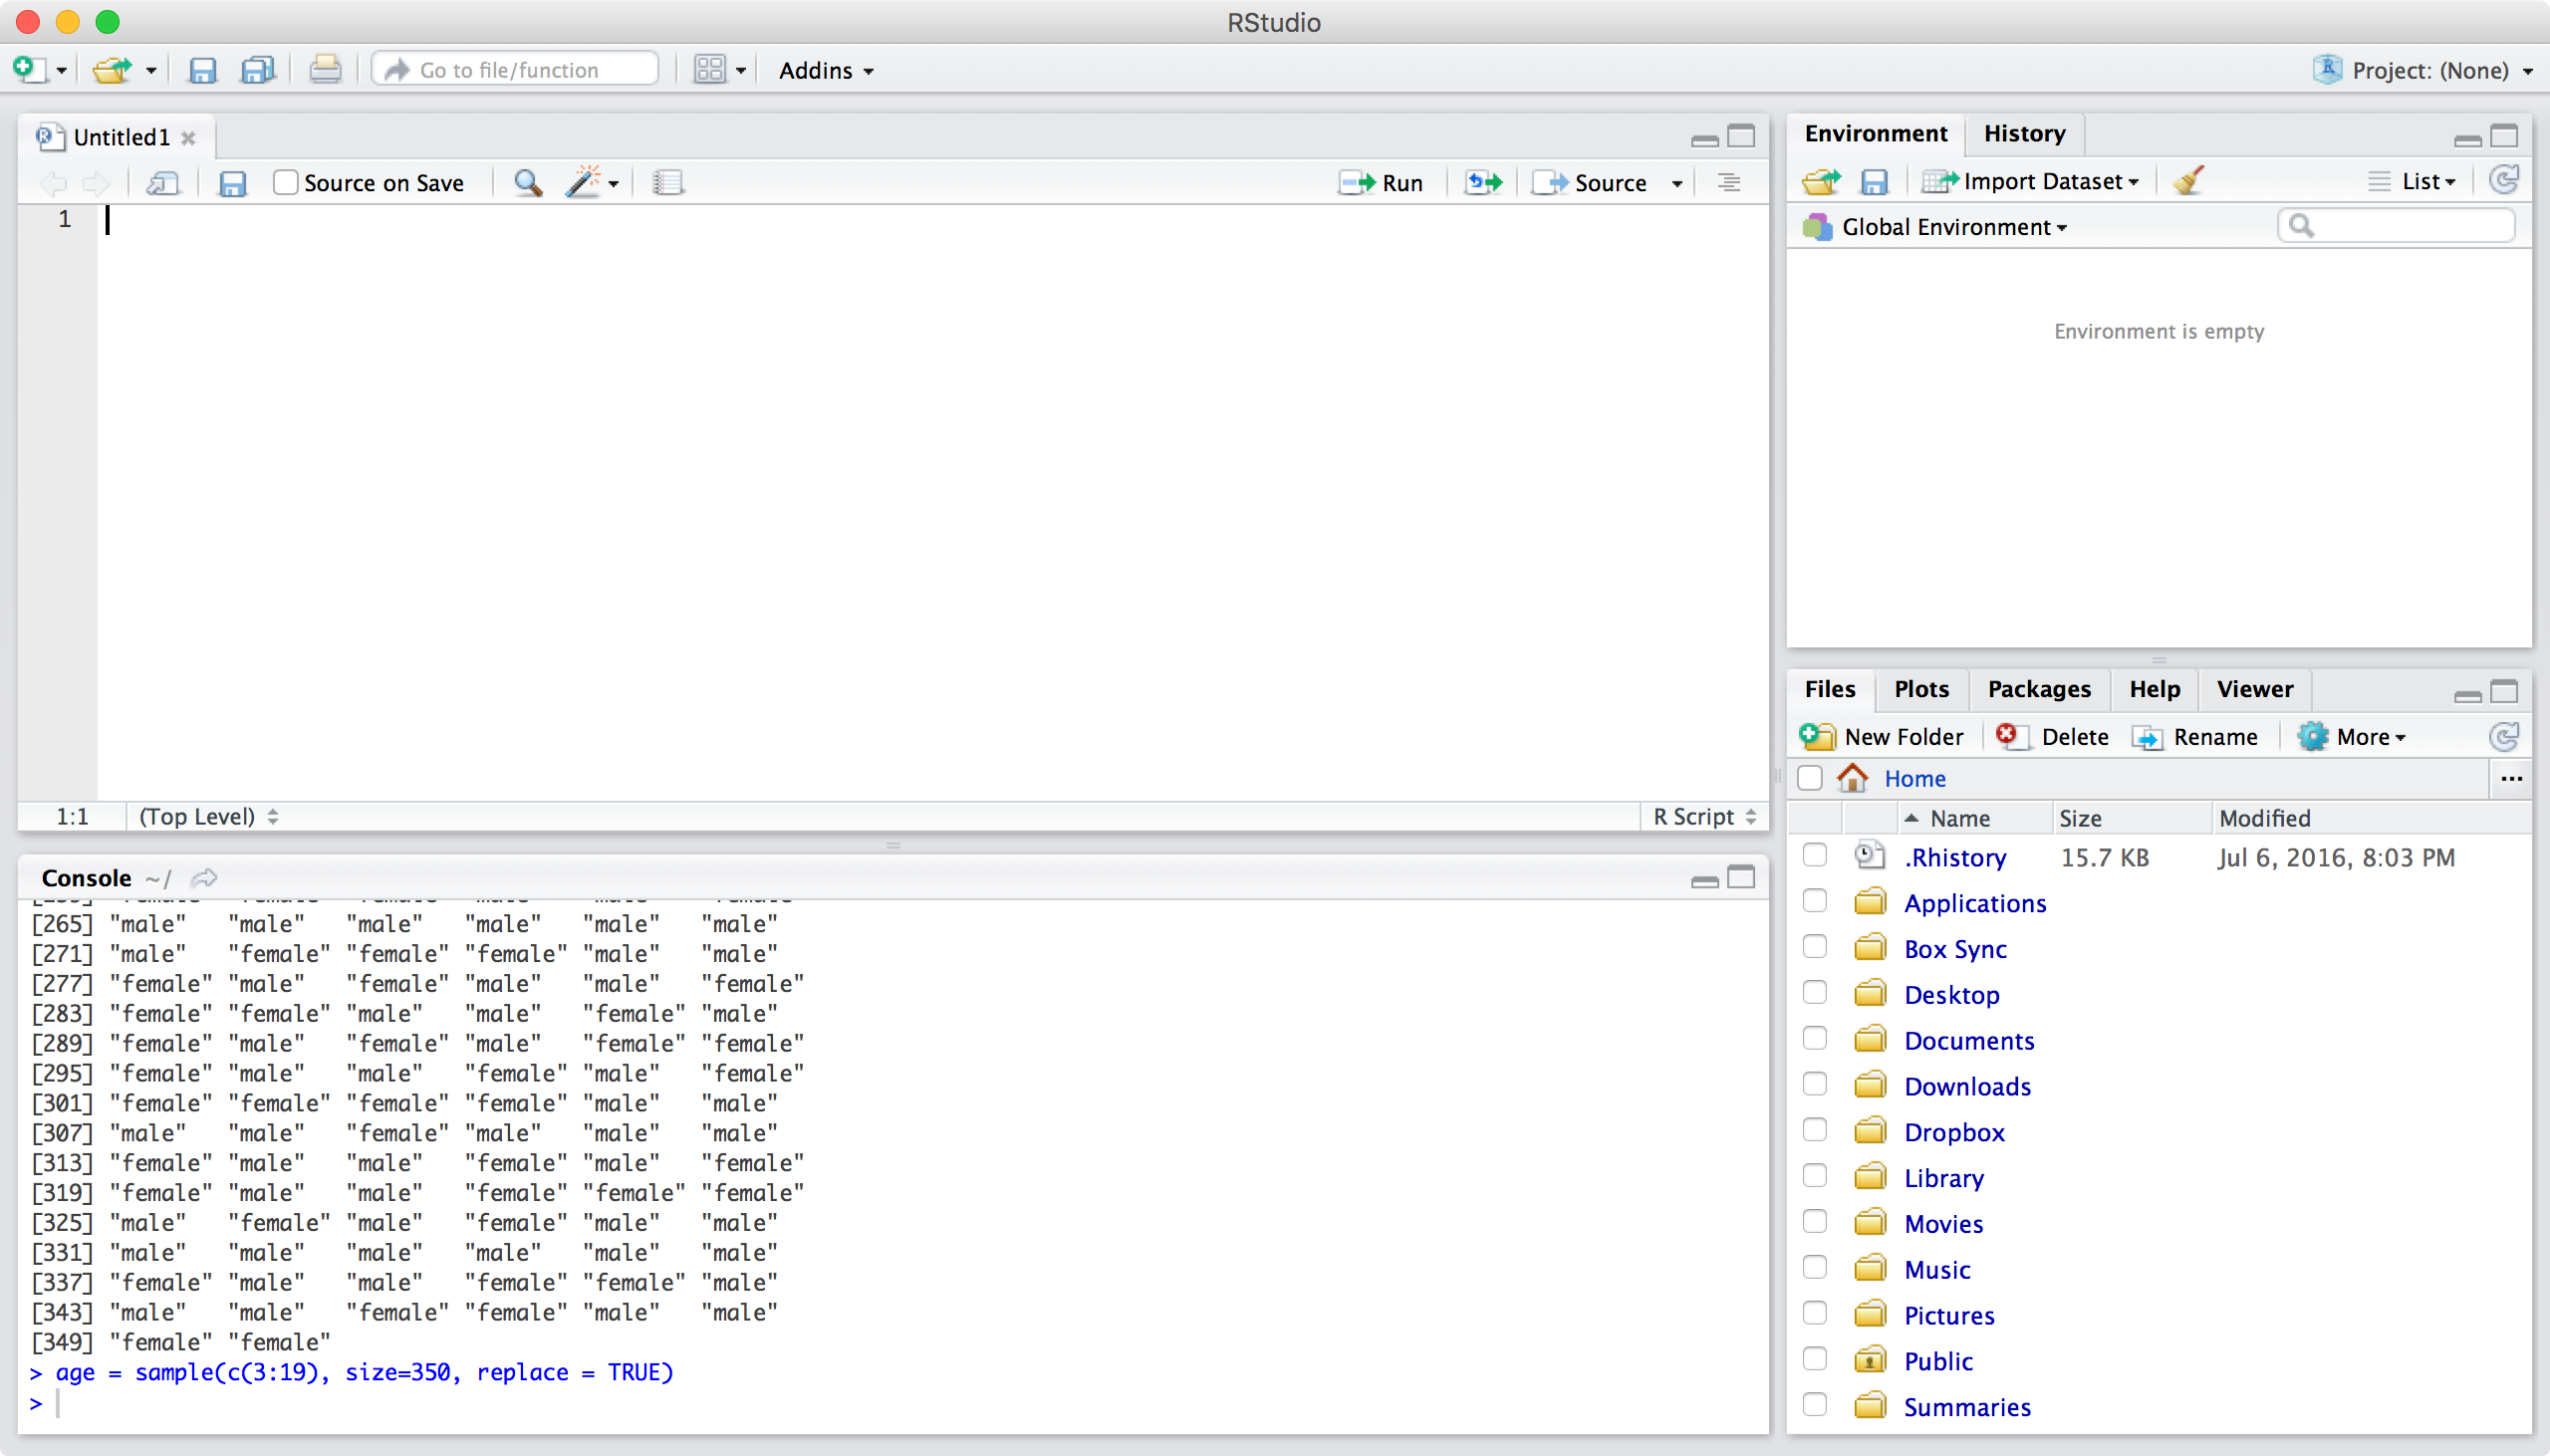
\includegraphics[width=180mm]{FourPanes.png}}
  \sidecaption{The Four Panes of RStudio}
  \label{fig_fourpanes}
\end{figure} 
The top left pane is the script pane. The bottom left is the consol pane. Top right pane has the environment and history. And finally, the bottom right pane has files, plots, packages and help.

\subsubsection*{Scripts}
When writing R code, it is best to write them in a script file\sidenote{\footnotesize There are other file types that you can use to write R code. We'll discuss others throughout the book, including Rmarkdown. But for now, a regular R script file is all you need}. These allow the code to be colored (for easier reading), autocomplete of code (which can be very useful), and it allows us to run the code right from the script using either the ``run" button at the top of the pane or using \texttt{command + enter} for a Mac (or \texttt{control + r} for a Windows).


\subsubsection*{Console}
The console pane is where the code is actually executed and the output is shown. Each time you run a line (or several lines) of code in a script file, the code will show in the console, the code will then be executed, and output will be displayed.

\subsubsection*{Environment and Files/Plots}
The other two panes (both the top and bottom panes on the right). In the top, the environment and history tab are both visible. The environment shows you any objects that are memory. These objects can be any type of R object that you've loaded\sidenote{\footnotesize This will become much more more clear in Chapter \ref{ch_tidy}. For now, just know that R works with objects, similar to the ones you have in the physical world. For example, a data object in R can be analyzed using many types of analyses but it can't create a plot on its own just like a chair in the physical world can be used to sit in or to stand on but you can't drive it to work on its own.} 

The bottom-right pane has several functions. When you create plots or figures it will show up there. It is also where, if you search for documentation on packages or functions, the documentation will be shown. There are other uses that we'll discuss later.


\subsection*{Data}
Data for the examples in this book can be loaded in R through several packages as well as a few data sets can found at \href{github.com/TysonStanley/R_Book}{GitHub}. Similarly, the R code used in this book can be downloaded there as well.


\subsection*{Data Analysis Steps}
A nice summary of the steps inherent in any data analysis can be found in Figure \ref{fig_steps}. Notice that the arrows point in both directions, suggesting that this is not a linear process but instead is very iterative. For example, cleaning the data may be one of the first things you do, and then you need to do it again after running some models.
\begin{marginfigure}
  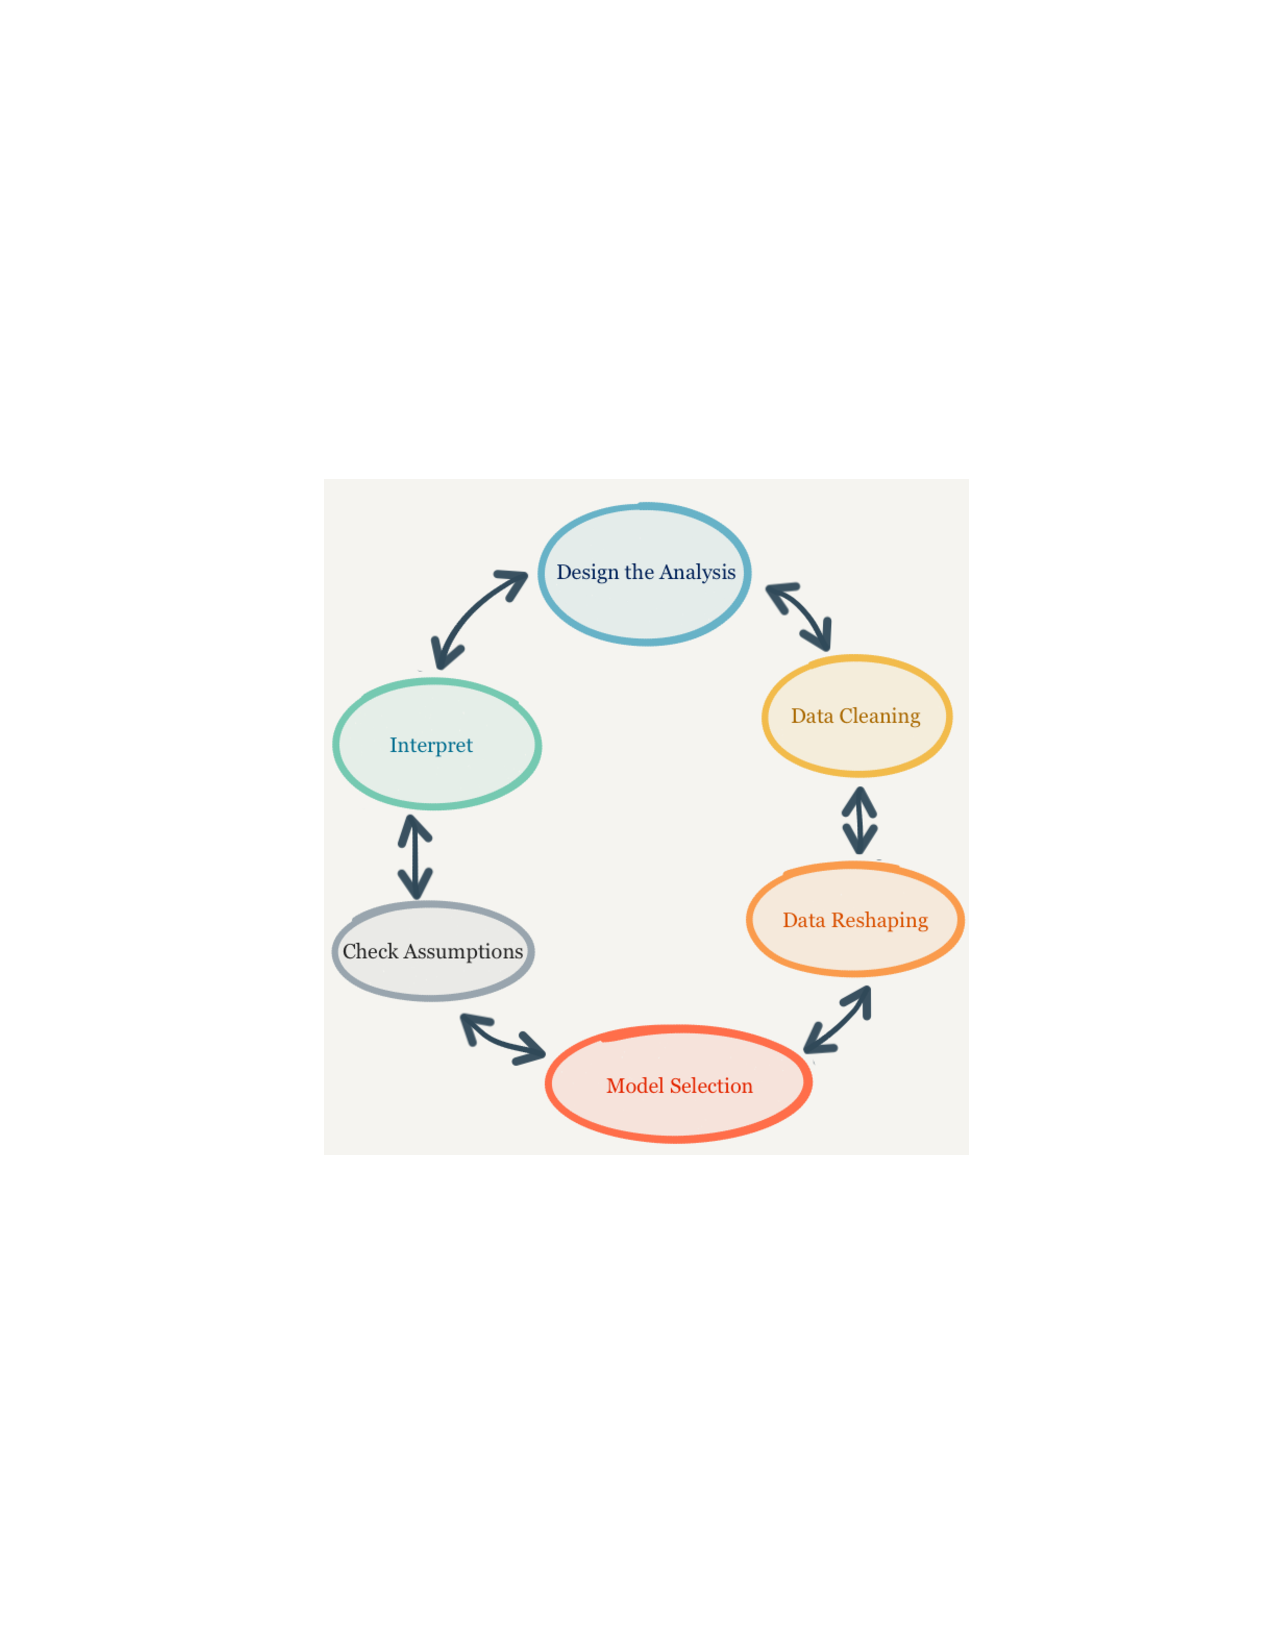
\includegraphics[width=50mm]{AnalysisSteps.pdf}
  \caption{Data analysis steps}
  \label{fig_steps}
\end{marginfigure}

At the top, ``Design the Analysis" is where any well-constructed data analysis starts. It is helpful to come up with an analysis plan that is actually written down. I've heard it often called a one-pager\sidenote{\footnotesize because it is good to keep it to one page since this forces you to keep things as simple as possible}. 

Next, ``Data Cleaning" is often where you earn your money during data analysis. If you are using real data, there is almost always problems. Relatedly, ``Data Reshaping" is all about getting the data into what we'll term ``tidy" form\sidenote{\footnotesize We'll discuss ``tidy" data in depth in Chapter \ref{ch_tidy}}, which allows easy analysis.

``Model Selection" and ``Check Assumptions" both are statistical in nature. Model selection is often theory driven but other methods, such as lasso regression and other machine learning tools, can help. This includes deciding what type of modeling can answer your questions (e.g., linear regression, logistic regression, mediation). This step also includes selecting what variables are of interest and what variables are needed to control for. After all this, we need to check our assumptions. Models are only good when they fit our data well, including the assumptions our models take on. \marginpar{\footnotesize This is a valuable life lesson as well. In any role, checking our assumptions often helps us avoid miscommuncation and avoidable mistakes. It also can help you avoid looking like an idiot.}

Finally, ``Interpret" is where both an understanding of the modeling technique you used and a capability to communicate the results in a meaningful way are necessary. It is here that as the researcher that you must communicate the story the data is telling. Ultimately, this is where all your hard work at designing, data cleaning and reshaping, and the modeling can pay off. If communicated well, your analyses can help shape intervention and policy.

As we go through the process of learning R, we will touch on, sometimes in depth, each of these steps. You'll see that as we do that R is very useful in all of them.

\subsection*{A Quick Intro to R's Language}

We will go through a quick introduction to R's language. There are several pieces that are important to distinguish:
\begin{enumerate}
\item Comments (for humans)
\item Functions that perform specific jobs
\item Assignment operators
\item Objects
\end{enumerate}
These pieces of code will become second nature to you pretty soon.

\subsubsection*{1. Comments Are For Humans}

\# is a comment. Put that before any line of code and the computer will ignore that it even exists. But you won't because it is likely that you are a human and will be able to continue to read the comment. These exist for two main reasons: 1) so you can keep track of what you are doing, and 2) to ignore some functions that you don't want to run at the present. For example:

\begin{Schunk}
\begin{Sinput}
> ## This symbol -- # -- is a comment, this will not be run
> ## I like to use two # for my comments
> ## Use comments to document what you are doing in your code
\end{Sinput}
\end{Schunk}

So if these lines are in my code, the computer won't even see them. But it can remind me of what I was thinking when I wrote the code or what my end goal might be. You'll see these plenty throughout the book.

\subsubsection*{2. Functions}

These are the money-makers for R. 

Hadley Wickham's description of a function...

Many functions are built into R. However, many other helpful functions can be downloaded and then loaded into R. The most common way of doing this is through the following functions:

\begin{Schunk}
\begin{Sinput}
> install.packages("dplyr")
> install.packages("tidyr")
> install.packages("haven")
> library(dplyr)
> library(tidyr)
> library(haven)
> 
\end{Sinput}
\end{Schunk}

\verb|install.packages()| downloads the package from CRAN (where the most tested and reliable packages are). This only needs to be done once for each package until you want to update. \verb|library()| loads the package into your R session. This needs to be done each time you use R.

These packages shown give us many tools to clean and tidy up our data. We will be using these three fairly extensively throughout the book. There are other great packages that we'll talk about as well.

\subsubsection*{3. Assignment}

There are two main assignment operators, as you can see in the code below:

\begin{Schunk}
\begin{Sinput}
> myobj <- something
> myobj = something
\end{Sinput}
\end{Schunk}

These, in most situations, do the exact same thing. The thing on the right is assigned to the thing on the left. Here we are assigning \verb|something| to \verb|myobj|. To understand this better, we need to talk about objects in R.

Note, to assign several objects to one name, we can use \verb|c()|. Below, both \verb|something| and \verb|another| are assigned to \verb|myobj|. 

\begin{Schunk}
\begin{Sinput}
> myobj <- c(something, another)
\end{Sinput}
\end{Schunk}

This will make more sense as we go through more examples in the ``Objects" subsection below.

\subsubsection*{4. Objects}

Objects in R are virtual objects that, like physical objects, are things that you can use to perform some function. For example, chairs are very useful to sit on or to stand on to reach something high, but they would be horrible to use as a vehicle to travel. Similarly, different R objects have different utility. Some objects are good to analyze, others are good to perform functions\sidenote{\footnotesize functions are a type of object but we'll keep them separate from the data objects we will be talking about}, and yet others may just be a single number.

When using R for health, behavioral, and social sciences, data objects are very important to understand. It is best to start at the smallest form of data and work our way up. There are four types of data vectors\marginpar{\footnotesize \textbf{Vector} refers to a column of data, which can often be seen as a single variable in a data set. It is comprised of at least one element but can have many elements, as most variables do.} that are commonly used:

\begin{enumerate}
\item Numeric
\item Factor
\item Character
\item Date
\end{enumerate}

Numeric objects have, shockingly, numbers. So a column of data about individuals' weights would be numeric if the values are in number units such as lbs or kg units (e.g., 150 lbs.). 

\begin{Schunk}
\begin{Sinput}
> weight <- c(150.1, 143.1, 182.2, 134.4)
\end{Sinput}
\end{Schunk}

Factor objects are categorial variables (i.e., ordinal or nominal variables). These can take on numeric categories (groups 1, 2, and 3) or string \marginpar{\footnotesize \textbf{String} is a collection of letters, often forming a word or a group of words} categories (groups "male" and "female").

\begin{Schunk}
\begin{Sinput}
> gender <- c(1, 2, 1, 2, 1, 2)
> gender <- c("male", "female", "male", "female", "male", "female")
\end{Sinput}
\end{Schunk}

Character objects have strings. It can have any string, and unlike factors, it doesn't assume a finite number of possible strings. These are less useful for many of the methods used in the health, behavioral, and social sciences. Instead, we'll use factors the most. However, at times this type of object can be very useful.

\begin{Schunk}
\begin{Sinput}
> char <- c("This is a string", "This is another string", "Interesting example")
\end{Sinput}
\end{Schunk}

Finally, date objects are special objects that contain a date (I know, again, it's quite shocking). These require a bit of telling \verb|R| that it is a date. The following code assigns \verb|obj| as a date with the format of MM/DD/YYYY. Once we've done that, we can calculate days between interventions, testings, or birth to intervention fairly easily.

\begin{Schunk}
\begin{Sinput}
> date <- as.Date(obj, "%m/%d/%Y")
\end{Sinput}
\end{Schunk}

Using these vectors, we can combine them into the ultimate object -- a date frame. A date frame is the format that you are likely use to. It is similar to the data you are used to in programs like SPSS and Excel. 

\begin{Schunk}
\begin{Sinput}
> weight <- c(150.1, 143.1, 182.2, 134.4)
> gender <- c("male", "female", "male", "female")
> char <- c("Jim", "Pam", "Tom", "April")
> data <- data.frame(weight, gender, char)
> data
\end{Sinput}
\begin{Soutput}
  weight gender  char
1  150.1   male   Jim
2  143.1 female   Pam
3  182.2   male   Tom
4  134.4 female April
\end{Soutput}
\end{Schunk}

As you can see, we combined the numeric, the factor, and the character vectors into a data.frame called data. We then print that object and we can see what is in it. For most of our analyses, this is how we'll want our data -- in a beautiful data frame.

There is one other data object that can be very useful. It is known as a list. The nice thing about a list is that each element (or thing within the list) can be anything. It doesn't have to match the previous or the subsequent elements in type or size.

\begin{Schunk}
\begin{Sinput}
> list1 <- list(data, "This is a string", c(1,1,3,2))
> list1
\end{Sinput}
\begin{Soutput}
[[1]]
  weight gender  char
1  150.1   male   Jim
2  143.1 female   Pam
3  182.2   male   Tom
4  134.4 female April

[[2]]
[1] "This is a string"

[[3]]
[1] 1 1 3 2
\end{Soutput}
\end{Schunk}

This example is a bit dumb, but there are times that using a list can save you a lot of time and energy. These moments often accompany things that need to be done many times. We'll talk about this more in later chapters.




\begin{Schunk}
\begin{Sinput}
> ## This symbol -- # -- is a comment, this will not be run
> ## I like to use two # for my comments
> ## Use comments to document what you are doing in your code
> 
> ## Need to install packages (only need to once) and 
> ##   load packages (load each time you open RStudio)
> ## These provide functions that you'll want
> ## An example of packages that we'll be using:
> 
> install.packages("dplyr")
> install.packages("tidyr")
> install.packages("haven")
> library(dplyr)
> library(tidyr)
> library(haven)
> ## Importing Data
> ##   1. For RData or rda files
> load()
> ##   2. For CSV files
> read_csv()
> 
> 
\end{Sinput}
\end{Schunk}






\chapter{R Can be Your Best Friend}
\label{ch_intro}

\textsc{Welcome} to the start of a best friendship. You may not know it yet, but the simple looking R program you've heard about has hidden beauty that is to die for. This beauty really comes out when it wears its best attire -- called RStudio\sidenote{\footnotesize We discussed how to download and install this in the Introduction. We'll discuss some of the awesome features of RStudio throughout the book.}.

It takes a little getting to know before a real best friendship with R can develop\sidenote{\footnotesize That, I guess, is true of any friendship}. But slowly, its best attributes begin to shine and you'll wonder why you ever spent time with another statistical software.

To be candid, this book is unlike most other R books or tutorials. For one, it is not designed to be comprehensive, throwing a large number of functions and methods at you. If you are a fairly normal human, I'd say once you've gotten a good start on learning R, you'll end up using the internet to answer most of your questions. Occasionally, you'll look in a comprehensive R book for advice. In my experience, individual questions answered over websites such as StackOverflow and R-bloggers often get at your question better than most books are able to\sidenote{\footnotesize Of course, there are exceptions to this}.

This book is designed for social scientists. Most books about R, on the other hand, address R in regards to data science since it is the hot job right now. You'll find all the books you need dealing with data science techniques in R. This makes sense since R is a powerful (possibly the most powerful) tool that a data scientist has. These methods are very useful for social scientists as well. However, given you are reading this book, you are probably not a data scientist and would rather know how you can use R for the methods you are currently needing to use. 

If you perform research or program evaluation in psychology, economics, political science, education or sociology then this book is a great resource to get you started on your road to becoming best friends with R. Then, if your love of R grows deep, you can explore more in depth R books\marginpar{\footnotesize See \href{http://adv-r.had.co.nz/}{Hadley Wickham's Advanced R (also available online)}, \href{https://www.amazon.com/ggplot2-Elegant-Graphics-Data-Analysis/dp/331924275X/ref=sr_1_1?s=books&ie=UTF8&qid=1467916355&sr=1-1&keywords=ggplot2}{Hadley's ggplot2 book}, \href{https://www.amazon.com/Introduction-Statistical-Learning-Applications-Statistics/dp/1461471370/ref=sr_1_3?s=books&ie=UTF8&qid=1467916072&sr=1-3&keywords=r+statistics}{An Introduction to Statistical Learning}}.

This means we will focus on the methods you will use the most, starting with data cleaning and management, exploratory and publishable graphics, and modeling. I am more concerned with you understanding what you can do and why you should do it than having you memorize code; that will come with experience and time.

\section*{What Makes R Such a Good Friend?}

Why am I so convinced you'll find R a fantastic friend? Simply, it has advantages in several key ways:

\begin{enumerate}
\item It is free. Does this need any further elaboration?
\item It is open-source, meaning anyone around the world can try to add to it. If this doesn't seem like an advantage, it will become clearer as we go through the amazing packages that people around the world have developed, once again, for free.
\item It is a programming language. This says that we can do just about anything with it.
\item There is a large community that can help. Simply searching the web regarding your questions often produces useful results.
\end{enumerate}
Of course, there are downsides to any good friend. In R's case: 
\begin{enumerate}
\item Since it is free, there is no warantee\sidenote{\footnotesize This has yet to be a big problem}.
\item Since it is open-sourced, there are many tools available that aren't that great. Sifting through them to find the one you need can be tiring\sidenote{\footnotesize There are helpful blogs on \href{https://github.com/}{GitHub} and other sites that are very helpful}.
\item There is a steep learning curve\sidenote{\footnotesize That's why I wrote this book}. 
\item Some tools aren't kept up to date by the developer and so they aren't useful anymore \sidenote{\footnotesize We'll learn about writing our own functions to perform things we need done that hasn't been deveoped openly yet in Chapter \ref{ch_functions}}
\end{enumerate}
It appears that I am a bit biased in favor of R. Full disclosure, R, nor any of its affiliates, are paying me. The only reason I am so in favor of R is because I've had experience with other stats software and, although many of these are very useful, none do quite what R can do.\sidenote{\footnotesize I also very much like Stata, SAS, and SPSS. Each do their specific things very well. If you are already using one of these and really like how they perform certain analyses (the ``margins" command in Stata is a good example), I recommend using R for most of your data cleaning and management, exploratory analyses, and plotting and then transfer your data to another package.}

\section*{What can R really do?}

But enough of the chit-chat. It is time to show off some of R's power. These are all things that I've personally done using R.

\subsection*{Graphics}

As we discussed previously, R has graphics that most other software could only dream of.

%% Insert figures here from previous data analyses


\subsection*{Documents}

R is a powerful tool for creating documents. In fact, this book was written in R. Several powerful packages create well-formatted PDF's, html, and word documents that can easily incorporate code, output, and text into one beautiful document or website. This is extremely useful in performing reproducible research since the code and text are all together. It is also useful in creating reports, especially if it is a repetitive task that needs to be reported on often. Although it may be strange to think of using a statistical package to write a paper, it is just one example of the wide-reaching abilities R contains.

\subsection*{Most Up-to-Date}

As statisticians develop new methods, many academic journals require that they release a way to apply the method. Since developing new methods and packages in R is so straightfoward and cheap and since R is a great way to provide it to a large group of people, many statisticians provide a new package for the method. This means R is often the most up-to-date stats software available. And, if you have already forgotten, it is free.

This also shows us that R is still improving. That's the power of being open-source. People all over the world are giving of their time and talents to make things easier for other R users like you and me. One of these individuals, Hadley Wickham, has created a host of packages that make our lives easier. He called the ideology of using well formed data, and the tools associated with that ideology, "Tidyverse".





\chapter{Tidyverse}
\label{ch_tidy}

\textsc{At the} UseR Conference in 2016, Hadley addressed the large number of tools he has created. Many have termed the group of tools as the ``Hadleyverse"\sidenote{\footnotesize A play on Hadley's Universe, just in case that wasn't clear}. He suggested we refer to it as ``Tidyverse" instead, referring to the ideal analyzable form of data (i.e.,``tidy" form). This way of thinking about data is very important in the social sciences.

First, it gives a firm framework of what kind of data we should collect in research. It also helps us understand what kind of questions you can ask with different forms and kinds of data. With that understanding, you can immediately be a better researcher.

There's two main forms of ``tidy" data: 1) wide format and 2) long format. We'll use an example to illustrate:

\subsection*{Long and Wide Format}

Using a fictitious dataset on the individuals, their economic characteristics, health status and health behaviors, we will illustrate long and wide format. Then we will show, using the \texttt{tidyR} package, how to take it from one form to the other.

\begin{Schunk}
\begin{Sinput}
> ## Need to install (only need to once) and 
> ##   load packages (load each time you open RStudio)
> 
> library(dplyr)
> library(tidyr)
> 
> ## Read in the Data
> 
> 
\end{Sinput}
\end{Schunk}


\subsection*{Dealing with Missingness}




\subsection*{}



\chapter{Quick Summaries of Your Data}
\label{ch_summaries}





\chapter{Exploratory Graphics}
\label{ch_expgraphics}



\chapter{Graphics That You Can Publish}
\label{ch_pubgraphics}


\chapter{Writing Your Own Awesome Functions}
\label{ch_functions}




\end{document}
